\documentclass[a4paper]{article}
\usepackage{enumerate}
\usepackage{amsmath}
\usepackage[english]{babel}
\usepackage{url}
\usepackage{graphicx}

\title{k-Nearest-Neighbours\\\large Lab Session 1\\Machine Learning: Pattern Recognition\\Master Artificial Intelligence}

\author{Camiel Verschoor \\StudentID: 10017321\\UvAnetID: 6229298\\ \url{Verschoor@uva.nl} \and Steven Laan\\StudentID: 6036031\\UvAnetID: 6036031\\\url{S.Laan@uva.nl}}

\begin{document}

\maketitle

\section{Data Visualization}
\begin{figure}[!ht]
\centering
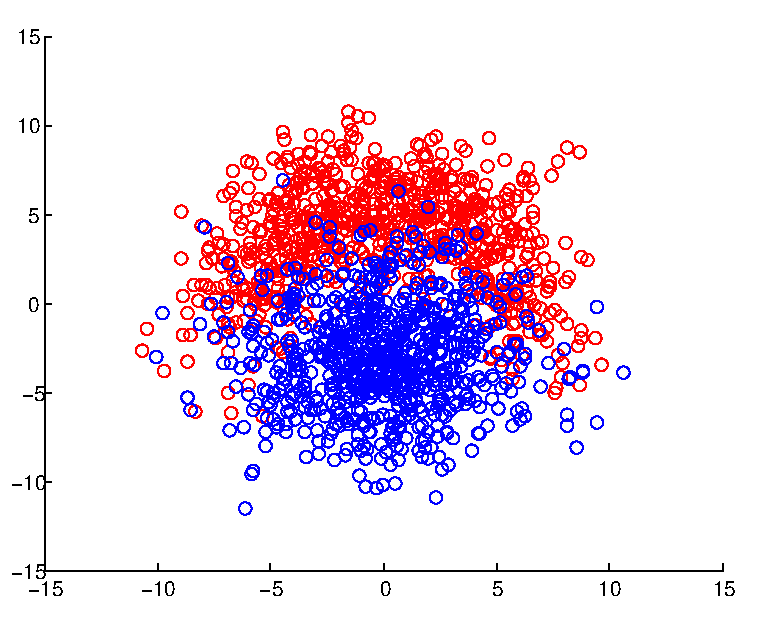
\includegraphics[width=0.75\textwidth]{images/data_scatterplot.pdf}
\caption{Data visualization}
\label{data}
\end{figure}
\section{k-Nearest Neighbours}

\section{Cross Validation}


\end{document}